\chapter{Uvod}
Diplomska naloga je ponovna implementacija in nadgradnja interaktivne
umetniške instalacije ``15 sekund slave''~\cite{15secLeonardo}. Motivacija za
instalacijo je umetniško delovanje ameriškega pop-art umetnika Andyja Warhola.
``15 sekund slave'' izgleda kot klasična slika, a je dejansko računalniški
zaslon, okvirjen kot umetniška slika. Nad zaslonom je v okviru vgrajen
digitalni fotoaparat, ki je povezan z računalnikom v ozadju. Vsakih 15 sekund
fotoaparat slika obiskovalce galerije, ki stojijo pred sliko. Na sliki
računalniški program poišče vse obraze in nato naključno izbere enega izmed
njih. Ta obraz nato z grafičnimi filtri program obdela tako, da pridobi tako
imenovani ``pop-art'' videz z manjšim številom živih barv, ki spominjajo na
slike slavnih osebnosti, ki jih je iz fotografij delal Andy Warhol. Ker je
prvotna instalacija nastala pred več kot 10 leti in se je strojna oprema v tem
času že zelo spremenila, se je pokazala potreba po prilagoditvi aplikacije
novemu stanju tehnologije \cite{trifonova}.

V magistrski nalogi najprej preučite splošne probleme pri vzdrževanju
umetniških instalacij, ki temeljijo na računalniški tehnologiji
\cite{miller1,miller2,digitalartconservation}. Zaradi hitrega napredka
računalniške tehnologije je potrebno take aplikacije po eni strani prilagajati
novi strojni in sistemski programski opremi, pa tudi novim funkcionalnim
možnostim, ki jih nove tehnologije nudijo. Po drugi strani, pa z umetniškega
vidika običajno želimo, da se zunanja pojava umetniškega dela ne spremeni. V
konkretnem primeru instalacije ``15 sekund slave'' namesto računalnika in
digitalnega fotoaparata uporabite mobilni telefon z vgrajeno kamero ter
možnostjo brezžičnega prenosa podatkov. V enem načinu delovanja nove
implementacije instalacije, se naj zunanji izgled, način uporabe in generirane
slike ne razlikujejo od prvotne instalacije. V drugem načinu delovanja nove
implementacije pa poiščite nove, kreativne načine funkcioniranja, ki jih
omogoča novejša tehnologija. Tu je mišljena predvsem uporaba videa namesto
statične slike in povezovanje s socialnimi omrežji.

\chapter{Andy Warhol}
Referenca~\cite{wiki:AndyWarhol}
\section{Pop-art umetnost}


\chapter{Prvotna izvedba: 15 sekund slave}
``15 sekund slave'' je interaktivna umetniška instalacija, ki obraz naključno
izbranega obiskovalca galerije povzdigne v umetniški objekt za petnajst
sekund. Instalacija je bila navdahnjena s slavnim citatom Andyja Warhola: ``V
prihodnosti bodo vsi ljudje doživeli svojih petnajst minut
slave''\footnote{Originalno v angleščini: \textit{``In the future everybody
will be world-famous for fifteen minutes''}\cite{andyExhibition}.} kot tudi z njegovim načinom
predelave obrazov v slogu pop-art~\cite{15secSlo}.


\section{Strojna in programska oprema}
Če pogledamo sliko~\ref{fig:15sec} vidimo le ``mojstrovino'', uokvirjeno v
dragocen okvir. Vendar pa je še veliko v ozadju, očem obiskovalcem nevidno.

\begin{figure}
    \centering
    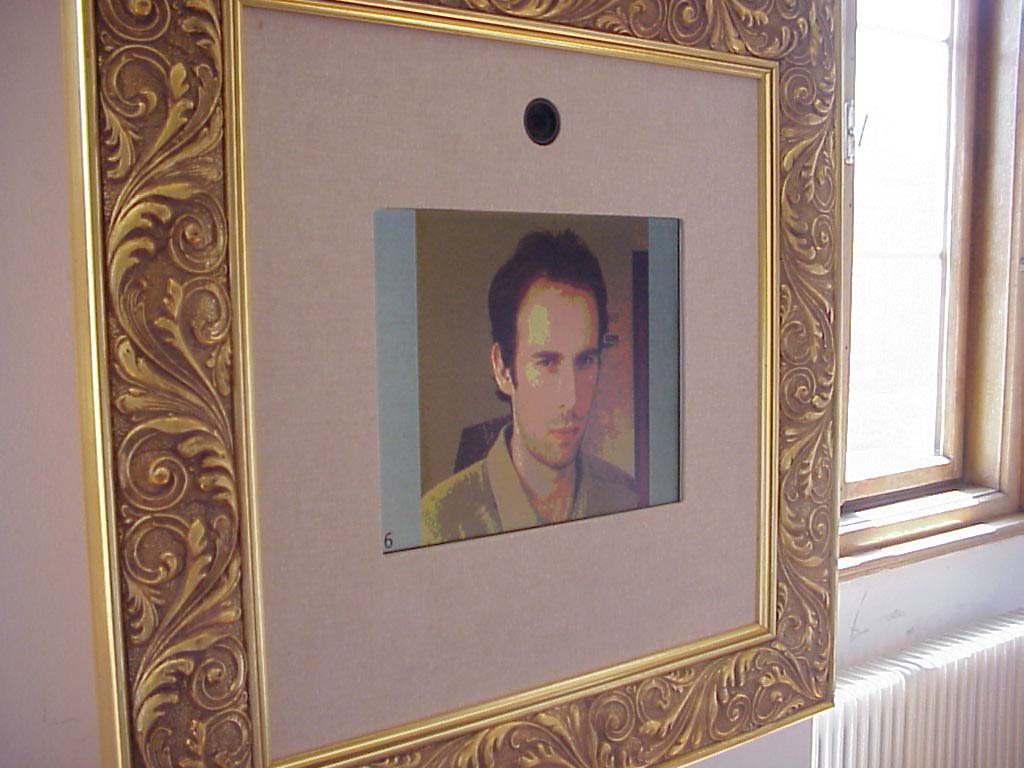
\includegraphics[width=0.7\textwidth]{15sec}
    \caption{Prikaz delovanja instalacije}
    \label{fig:15sec}
\end{figure}

Črna luknja nad notranjo sliko je prostor za digitalni fotoaparat, ki enkrat
na vsake petnajst sekund slika okolico ter sliko pošlje računalniku, ki je
tudi skrit v ozadju. Fotoaparat ima širokokoten objektiv, da lahko zajamemo
čim širšo okolico.

Kot že prej omenjeno, se slika pošlje računalniku. Na računalniku se najprej
izvede algoritem za iskanje obrazov. V primeru več najdenih zadetkov uporabimo
naključnega. Ta obraz izrežemo iz slike ter ga pošljemo naprej.

Dobljen obraz se obdala z enim izmed vnaprej določenimi barvnimi filtri. Ti
filtri so sestavljeni iz različnih barvnih transformacij, da vrnejo sliko v
slogu pop-art. Pop-art filtri so bolj podrobno opisani v
poglavju~\ref{ch:obdelavaSlik}, primer pop-art transformacije pa lahko tudi
vidimo na sliki~\ref{fig:lena_filter_5}.

Slika obraza v slogu pop-art, je končni rezultat, ki je prikazan takoj, ko
prejšnjemu obrazu poteče njegovih petnajst sekund. Prikazan kako? Notranja
slika obraza je v bistvu računalniški zaslon LCD, priklopljen na že prej
omenjeni računalnik.

Ta postopek se ponavlja v neskončnost, najboljše pa je, da se vse dogaja v
živo. Če bo nekdo dovolj dolgo gledal v okvir, ima veliko možnosti da bo kmalu
zagledal samega sebe kot ``mojstrovino'' v galeriji.

\chapter{Nadgradnja: Naprava in pripomočki}
Kot prvo nadgradnjo, ki smo si jo zamislili je čimbolj učinkovito zmanjšati
porabljen prostor za instalacijo in s tem povečati njeno prenosljivost in
enostavno postavitev.

Prvotna instalacija potrebuje osebni ali prenosni računalnik, zaslon LCD,
digitalni fotoaparat, mrežno opremo in dostop do interneta.

Kot najboljša zamenjava se je izkazala naprava ``pametni telefon'', saj
vsebuje vse prej naštete naprave. Ima vgrajeno kamero, ki služi tudi kot
fotoaparat, dostop do interneta preko kartice SIM ter operacijski sistem, ki
omogoča izdelavo programske opreme s katero lahko dostopamo do prej naštetih
funkcij.

Pametni telefoni dražjega ranga omogočajo tudi, da lahko sliko v živo
predvajamo na večji ekran. Zato smo se odločili, da kot testno napravo vzamemo
pametni telefon Samsung Galaxy S5.

\section{Testna naprava: Samsung Galaxy S5}
Samsung Galaxy S5 je pametni telefon, narejen v podjetju Samsung. Deluje na
operacijskem sistem Android verzije 4.4.4, imenovan tudi Android Kitkat.
Trenutno najnovejši operacijski sistem Android je verzija 5.0, poimenovan
Lizika (\textit{angl. Lolipop}).

TODO: opis naprave

Glavni razlog, da smo se odločili za to napravo je kvalitetna kamera, zmogljiv
procesor ARM in možnost priključka zunanje naprave prek priključka HDMI. 

Pomembna lastnost je tudi operacijski sistem Android, za katerega je mogoče
napisati programsko opremo, imenovano aplikacija, v programskem jeziku Java.
Vse kar za to potrebujemo je Android SDK in prevajalnik Java.


\section{Android}
Android je odprtokodni sistem za pametne telefone, ki ga je izdelal Open
Handset Alliance pod vodstvom podjetja Google, leta 2007. Projekt se imenuje
AOSP~\footnote{Celotno ime je Android Open Source Project} in se še danes
hitro razvija.

Vse skupaj temelji na jedru Linux, najbolj bistven del arhitekture pa je
navidezni stroj (\textit{angl. virtual machine}). Bolj podrobna zgradba
sistema je prikazana na sliki~\ref{picAndroid}. Navidezni stroj, imenovan
Dalvik virtual machine, vsebuje prevajalnik JIT, ki je zadolžen za zaganjanje
že prevedene programske kode Java. Prevedena koda je zapakirana v datoteke s
končnico .apk in tej datotekam pravimo aplikacija, izdelana za sistem Android.

\begin{figure}
    \centering
    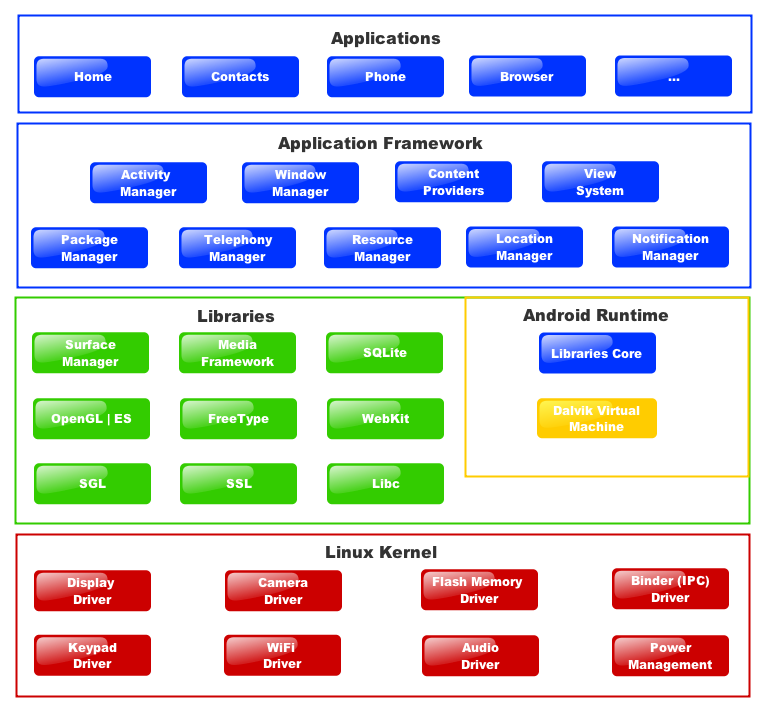
\includegraphics[width=\textwidth]{android}
    \caption{Struktura operacijskega sistema Android~\cite{wiki:Android}}
    \label{picAndroid}
\end{figure}

Za izdelavo aplikacije Android potrebujemo znanje programskega jezika Java,
Android SDK, ki je brezplačno na voljo na uradni spletni
strani\footnote{Uradna spletna stran je dostopna na {\tt
http://developer.android.com/}}, priporočljivo je tudi branje {\tt SDK}
dokumentacije, ki je na voljo na spletu\footnote{SDK dokumentacija je dostopna
na {\tt http://developer.android.com/sdk/}}. Dokumentacija je napisana
razločno, tako da se lahko znajdejo tudi začetniki. S pomočjo Android SDK na
koncu nastane datoteka .apk.

\chapter{Nadgradnja: Zaznavanje obrazov}
Operacijski sistem Android nam preko vmesnika JNI tudi omogoča vključevanje programskega jezika C. To nam omogoča uporabo splošnih knjižnic in programskih ogrodij (\textit{angl. framework}).

Ker smo v naši nadgradnji želeli, da bi se obrazi zaznavali v realnem času, smo se odločili za uporabo programskega ogrodja OpenCV.

\section{Zaznavanje obrazov z uporabo OpenCV}
OpenCV je programsko ogrodje, ki nam omogoča razne operacije nad slikami.
Napisana je v programskem jeziku C, za potrebe operacijskega sistema Android
pa so napisani povezovalni Java razredi (\textit{angl. class}), ki nam
omogočajo uporabo OpenCV operacij kar preko programskega jezika Java.

Najbolj pomembna funkcionalnost programskega ogrodja OpenCV nam je bila
implementacija zaznavanja obrazov. Uporablja algoritem kaskadnega
klasificiranja (\textit{angl. cascade classifier}), ki nam omogoča
klasifikacijo različnih lastnosti.

Lastnosti so zapisane v datoteki XML. Ta datoteka vsebuje več sto ali tisoč
različnih lastnosti, ki opisujejo določen predmet, kar v našem primeru pomeni
oblika obraz.

Obstajajo več različnih tipov, kako so te lastnosti opisane. Za zaznavanje
obrazov sta najpomembnejša tipa ``HAAR'' in ``LBP''. Tipa se razlikujeta po
točnosti in hitrosti.

``HAAR'' opisi so procesorsko bolj potratni in potrebujejo relativno veliko
časa za prepoznavo obraza, vendar pa je zato veliko manj napačnih detekcij
(\textit{angl. false positive}).

``LBP'' pa, čeprav z malo več napakah pri klasifikaciji, še vedno dovolj
točen. Vendar pa je časovno kar nekaj krat hitrejši od opisov ``HAAR'' in zato
zelo uporaben pri detekciji obrazov v živo.

Ker pa so obrazi med seboj zelo različni, je nemogoče da je vsak obraz najden,
hočemo pa, da je število zgrešenih čim manjše. Vendar pa zgrešen obraz ni
največja težava, saj gledalci tega ne bi opazili. Veliko večja težava je, če
najdemo obraz kjer ga ni. Na primer, kakšen predmet v okolici.

Testirali smo oba tipa, z različnimi tipi lastnosti. Uporabili smo le
lastnosti, ki opisujejo sprednji del obraza. Vendar pa se je pri uporabi
``LBP'' opisov še vedno pokazalo preveč lažnih obrazov. Zato smo se odločili
za uporabo lastnosti tipa ``HAAR''. Veliko bolj nam je pomembno, da ima
petnajst sekund slave obraz in ne kakšen predmet v okolici.

Vendar pa tudi tipi ``HAAR'' opisi obrazov niso vedno dosegli našega
pričakovanja. Zato smo se odločili, da naredimo dvojno klasifikacijo.

Najprej smo klasificirali z lastnostmi sprednjega dela obraza, opisanimi v datoteki
\textit{harrcascade\_frontalface\_default.xml}~\ref{lst:haar_frontal_face}, s
katero smo dobili rezultate obrazov. Ker je že sama klasifikacija obraza
porabila kar nekaj dragocenega časa, smo se odločili, da iskanje prekinemo po
prvem kandidatu obraza, ki je velik vsaj ena desetina celotne slike.

\begin{lstlisting}[label=lst:haar_frontal_face, caption=Izsek iz datoteke harrcascade\_frontalface\_default.xml]
<maxWeakCount>9</maxWeakCount>
<stageThreshold>-5.0425500869750977e+00</stageThreshold>
<weakClassifiers>
  <_>
    <internalNodes>
      0 -1 0 -3.1511999666690826e-02
    </internalNodes>
    <leafValues>
      2.0875380039215088e+00 -2.2172100543975830e+00
    </leafValues>
  </_>
  <_>
    <internalNodes>
      0 -1 1 1.2396000325679779e-02
    </internalNodes>
    <leafValues>
      -1.8633940219879150e+00 1.3272049427032471e+00
    </leafValues>
  </_>
  ...
\end{lstlisting}

Kandidat obraza smo testirali še s klasifikacijo očesa. Vsak obraz ima dve
očesi. Zavedali smo se, da v primeru očal tega ne bomo našli, vendar pa se je
izkazalo da je problem le pri zasenčenih očalih. Za to klasifikacijo smo
uporabili lastnosti, zapisane v datoteki
\textit{harrcascade\_eye.xml}~\ref{lst:haar_eye}. V primeru, če smo
našli točno dva rezultata smo vrnili prejšnji rezultat, v nasprotnem primeru
pa, da obraz ni najden.

\begin{lstlisting}[label=lst:haar_eye, caption=Izsek iz datoteke harrcascade\_eye.xml]
<maxWeakCount>6</maxWeakCount>
<stageThreshold>-1.4562760591506958e+00</stageThreshold>
<weakClassifiers>
  <_>
    <internalNodes>
      0 -1 0 1.2963959574699402e-01
    </internalNodes>
    <leafValues>
      -7.7304208278656006e-01 6.8350148200988770e-01
    </leafValues>
  </_>
  <_>
    <internalNodes>
      0 -1 1 -4.6326808631420135e-02
    </internalNodes>
    <leafValues>
      5.7352751493453979e-01 -4.9097689986228943e-01
    </leafValues>
  </_>
  ...
\end{lstlisting}

S temi nastavitvami in omejitvami smo dosegli pričakovane rezultate. Najden
rezultat smo povečali še za približno eno tretjino, tako da je bil rezultat
kvadratne oblike. Zakaj eno tretjino? Iskali smo prednji del obraza in ga tudi
našli. Vendar v okvirju si želimo videti celotno glavo in ne samo obraza.
Povečava za eno tretjino se je izkazala kot ravno pravšnja za večino
testiranih primerov.

Detekcija obrazov z programskim ogrodjem OpenCV je le ena izmed možnosti, ki
smo si jih podrobneje ogledali. Kot prva implementacija je bila izbrana zaradi
velike kontrole nad vsakim korakom, kot so: detekcija obraza, določanje regije
kje iskati, detekcija oči v določeni regiji in še bi lahko naštevali.

Kljub zadovoljivimi rezultati iskanja obrazov, se je izkazalo, da slike
velikokrat niso ostre. Prej smo omenili, da imamo veliko kontrolo nad
različnimi algoritmi za detekcijo, kar pa ne pomeni za uporabo kamere, ki je v
pametnem telefonu. OpenCV uporablja sliko iz kamere tako kot je, brez
predhodne izostritve. Z drugimi besedami povedano, to uporablja kot kamero in
ne kot digitalni fotoaparat.


\section{Zaznavanje obrazov z uporabo Android SDK}
Android SDK je popolnoma druga zgodba kot pa OpenCV. Tukaj ni nobene kontrole in raznih parametrov, le v naprej določen algoritem.

Algoritem bazira na algoritmu NV1-NORM~\cite{nevenFaceRecognition}, ki ga je
izdelalo podjetje Neven Vision~\ref{fig:neven_vision}. Leta 2006 je Neven
Vision postalo last podjetja Google in se uporablja za zaznavo obraza v
različnih programih, ki jih je izdelalo podjetje Google, na primer program za
prikaz slik Google Picassa.

\begin{figure}[!ht]
    \centering
    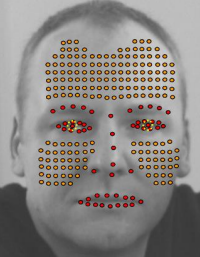
\includegraphics[width=0.3\textwidth]{neven_vision}
    \caption{Vizualizacija zaznavanja obraza, Neven Vision}
    \label{fig:neven_vision}
\end{figure}

Natančnejša implementacija algoritma za zaznavo obraza je zaprto-kodna. Tudi,
če si ogledamo dokumentacijo Android SDK-ja, je opisan samo primer uporabe:
\begin{lstlisting}[caption="Primer uporabe zaznavanja obraza z orodjem Android SDK"]
FaceDetector fc = new FaceDetector(
    sirina_slike,
    visina_slike,
    maksimalno_stevilo_obrazov
).findFaces(slika, obrazi);
\end{lstlisting}


\chapter{Nadgradnja: Obdelava slik}
\label{ch:obdelavaSlik}
Instalacija ``15 sekund slave'' vsebuje 17 različnih
filtrov~\cite[Poglavje~5]{thesisSamoJuvan} za obdelavo prejetih slik v
pop-art slike. Filtri so bili izdelani s pomočjo grafičnega programa GIMP.


\section{GIMP}
GIMP je odprto-kodno programsko orodje za obdelavo slik.


\subsection{Zgodovina}
Začetek projekta sega v leto 1995, kot semestrski projekt v Univerzi
Kalifornije, Berkeley. Kot prva avtorja, Spencer Kimball in Peter Mattis sta
projekt poimenovala \textit{angl. General Image Manipulation Program}. Malo
kasneje, ko je univerzo obiskal Richard Stallman sta ga prosila, če lahko
zamenjata besedo ``General'' v ``GNU''. Od takrat naprej se program imenuje
\textit{angl. GNU Image Manipulation Program} ali na kratko še vedno
GIMP~\cite{wiki:GIMP}.


\section{Izbira filtrov}
Že prvotna izbira filtrov je izhajala iz programskega orodja za predelavo slik
GIMP. Zaradi lažjega dela se je najprej grafičnega vmesnika izbralo zaporedje
različnih filtrov z različnimi parametri. Izbrani so bili naslednji filtri:
\begin{itemize}
    \item \textbf{uravnovešanje barv} \textit{angl. color balance} \hfill \\
        Prekrije celotno sliko z barvo v izbranem odtenku.
    \item \textbf{posteriziranje} \textit{angl. posterize} \hfill \\
        Zmanjšuje število barv na sliki.
    \item \textbf{uravnovešanje barv v HSL prostoru} \textit{angl. hue saturation balance} \hfill \\
        Spreminja odtenke barv, svetlost in intenzivnost na sliki.
\end{itemize}


\section{Implementacija filtrov}
Ker je GIMP odprto-koden smo imeli tudi dostop do implementacije filtrov.
Implementacije filtrov so napisani v programskem jeziku C. Na prvi pogled kot
nalašč za enostaven prenos na Android platformo preko JNI. Vendar pa so se
pokazale težave, saj so bili filtri močno povezani z GIMP objekti ter nekoliko
bolj kompleksni, kot smo mi potrebovali. Zato smo se odločili, da vzamemo samo
algoritem oziroma idejo za tem, ter implementiramo po naših potrebah. Naredili
smo tri različne implementacije in jih med seboj primerjali.

Prva implementacija je napisana v programskem jeziku java. Izkazalo se je kot
zelo počasno. Orodje za sproščanje pomnilnika GC \textit{(angl. garbage
collector)} se je klical velikokrat, kar je posledično porabilo več kot nekaj
sekund za filter. Tega si nismo mogli privoščiti, zato smo iskali alternative.

Naslednja implementacija je napisana s pomočjo grafične kartice in sicer z
orodjem OPENGL ES, verzije 2.0. Čas porabe pri izvajanju se je občutno
zmanjšal. Ko so bile teksture zapisane na grafični kartici so se filtri
izvajali v manj kot sekundi. Ta rešitev je bila že dovolj dobra, vendar pa se
nam je zdelo, da je uporaba grafične kartice za tako lahke operacije potrata
energije.

Čeprav so bili rezultati že dovolj dobri, smo se odločili še za implementacijo
v programskem jeziku C. Rezultati so pokazali, da je ta rešitev malo bolj
počasna kot prejšnja, vendar pa za to nismo potrebovali grafične kartice na
telefonu. Čas porabe je bil manj kot sekundo za filter.

\subsection{HSL barvni prostor}
\label{sec:hsl}

\begin{align}
R, G, B &\in [0,255] \nonumber \\
Cmax &= max(R, G, B) \\
Cmin &= min(R, G, B) \\
\Delta &= (Cmax - Cmin)
\end{align}

\begin{equation}
L = (max + min) / 2 \label{eq:hsl_l}
\end{equation}

\begin{equation}
S =
\begin{cases}
    0 \text{,}& \Delta = 0 \\
    255 * \Delta / (Cmax + Cmin) \text{,}& L < 128 \\
    255 * \Delta / (511 - Cmax - Cmin) \text{,}& \text{ostalo}
\end{cases}
\end{equation}

\begin{equation}
H' =
\begin{cases}
    0 \text{,}& \Delta = 0 \\
    0 + 42.5 * (G - B) / \Delta \text{,}& R = Cmax \\
    85 + 42.5 * (B - R) / \Delta \text{,}& G = Cmax \\
    170 + 42.5 * (R - G) / \Delta \text{,}& B = Cmax
\end{cases}
\end{equation}

\begin{equation}
H =
\begin{cases}
    H' + 255 \text{,}& H' < 0 \\
    H' - 255 \text{,}& H' > 255 \\
    H' \text{,}& \text{ostalo}
\end{cases}
\end{equation}

\begin{lstlisting}[caption=algoritem]
Cmax = max(R, G, B)

\end{lstlisting}

\subsection{Uravnovešanje barv}

\begin{equation}
clamp_{min}^{max}(x) =
\begin{cases}
    min \text{,}& x < min \\
    max \text{,}& x > max \\
    x \text{,}& \text{ostalo}
\end{cases}
\end{equation}

\begin{align}
shadows(x) &= clamp_{0}^{1}(\frac{117 - x}{64}) * 1.785 \\
color\_balance(x, x') &= clamp_{0}^{255}(x + x' * shadows(x)) \label{eq:color_balance}
\end{align}

Uravnovešanje barv se računa v barvnem prostoru RGB. Računamo jo za vsako
barvo posebej, in sicer z enačbo~\eqref{eq:color_balance}, kjer je $x$ enak
originalni barvi, $x'$ pa barvi, s katero želimo uravnovesiti originalno barvo
$x$. $x$ in $x'$ sta pozitivni celi števili med 0 in 255.

Po izračunanih vrednosti dane rezultate v RGB prostoru prenesemo v HSL prostor
s pomočjo enačb, napisnih v poglavju~\ref{sec:hsl}. Tako dobimo $H$, $S$ in
$L$. Iz originalnih vrednosti, to je vrednost barve na sliki, izračunamo
$L$~\ref{eq:hsl_l} in ga nadomestimo s prejšnjim, zato da ohranimo podobno
svetlost. $H$, $S$ in novo pridobljeni $L$ spremenimo nazaj v RGB prostor.

\subsection{Posteriziranje}

\begin{equation}
luts(x, levels) = 255 * \frac{\left \lfloor{\frac{x}{255} * (levels - 1) + 0.5}\right \rfloor}{levels - 1} + 0.5
\end{equation}

Posteriziranje se računa v barvnem prostoru RGB...

\subsection{Uravnovešanje barv v HSL prostoru}

\begin{align}
htv(x, x') &= x + 255 * \frac{x'}{360} \nonumber \\
hue\_transfer(x, x') &=
\begin{cases}
    htv(x, x') + 255 \text{,}& htv(x, x') < 0 \\
    htv(x, x') - 255 \text{,}& htv(x, x') > 255 \\
    htv(x, x') \text{,}& \text{ostalo}
\end{cases}
\end{align}

\begin{align}
ltv(x, x') &= clamp_{-255}^{255}(1.27 * x') \nonumber \\
lightness\_transfer(x, x') &=
\begin{cases}
    x * \frac{255 + ltv(x, x')}{255} \text{,}& ltv(x, x') < 0 \\
    x + \frac{(255 - x) * ltv(x, x')}{255} \text{,}& ltv(x, x') \geq 0
\end{cases}
\end{align}

\begin{align}
stv(x, x') &= clamp_{-255}^{255}(2.25 * x') \nonumber \\
saturation\_transfer(x, x') &= clamp_{0}^{255}(x + x * \frac{stv(x, x')}{255})
\end{align}

\subsection{Sestavljanje pop-art filtrov}

\subsubsection*{Filter 1}
Prvi filter je sestavljen iz dveh osnovnih filtrov. Najprej sliko obdelamo s
filtrom ``uravnovešanje barv'' in sicer s parametri $R = 30$, $G = -32$ in
$B = 16$. Rezultat obdelamo še s filtrom ``posteriziranje'' s parametrom
$ST =4$. Rezultat testne slike lahko vidimo na sliki~\ref{fig:lena_filter_1}.

\begin{figure}[!ht]
    \centering
    \begin{subfigure}[b]{0.4\textwidth}
        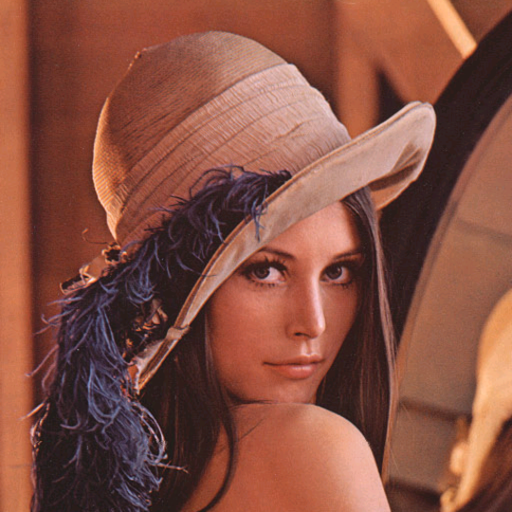
\includegraphics[width=\textwidth]{lena}
        \caption{Original}
    \end{subfigure}
    \begin{subfigure}[b]{0.4\textwidth}
        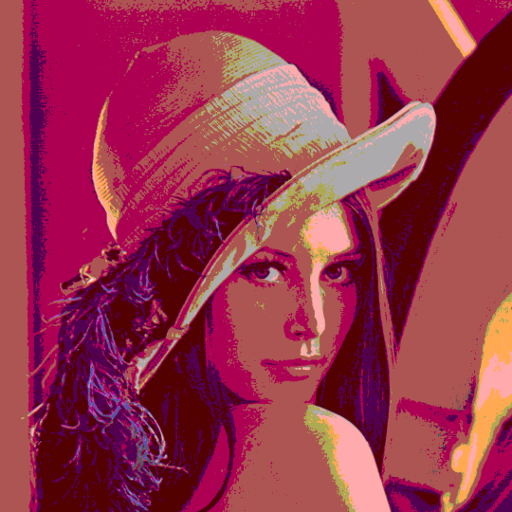
\includegraphics[width=\textwidth]{lena_filter_1}
        \caption{Prvi filter}
    \end{subfigure}
    \caption{Primerjava originalne slike z obdelano sliko}
    \label{fig:lena_filter_1}
\end{figure}


\subsubsection*{Filter 2}
Drugi filter je sestavljen iz dveh osnovnih filtrov. Najprej sliko obdelamo s
filtrom ``uravnovešanje barv'' in sicer s parametri $R = -36$, $G = -37$ in
$B = 39$. Rezultat obdelamo še s filtrom ``posteriziranje'' s parametrom
$ST = 4$. Rezultat testne slike lahko vidimo na sliki~\ref{fig:lena_filter_2}.

\begin{figure}[!ht]
    \centering
    \begin{subfigure}[b]{0.4\textwidth}
        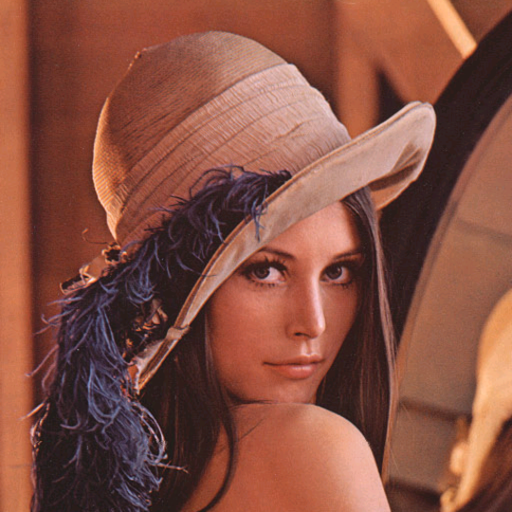
\includegraphics[width=\textwidth]{lena}
        \caption{Original}
    \end{subfigure}
    \begin{subfigure}[b]{0.4\textwidth}
        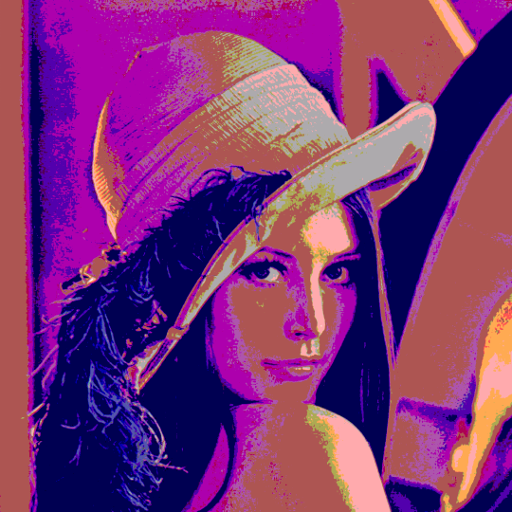
\includegraphics[width=\textwidth]{lena_filter_2}
        \caption{Drugi filter}
    \end{subfigure}
    \caption{Primerjava originalne slike z obdelano sliko}
    \label{fig:lena_filter_2}
\end{figure}


\subsubsection*{Filter 3}
Tretji filter vsebuje le osnovni filter ``posteriziranje'' in sicer s parametrom
$ST = 2$. Rezultat testne slike lahko vidimo na sliki~\ref{fig:lena_filter_3}.

\begin{figure}[!ht]
    \centering
    \begin{subfigure}[b]{0.4\textwidth}
        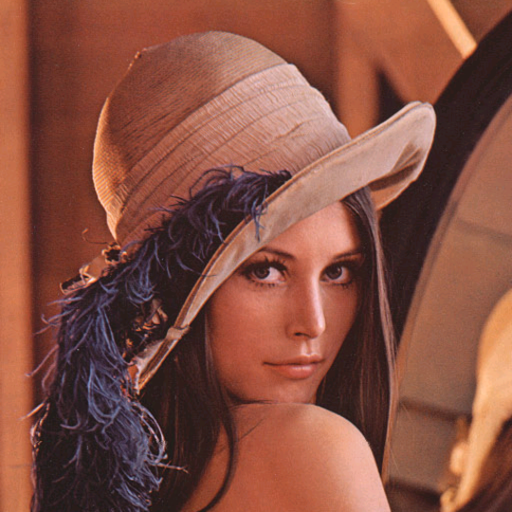
\includegraphics[width=\textwidth]{lena}
        \caption{Original}
    \end{subfigure}
    \begin{subfigure}[b]{0.4\textwidth}
        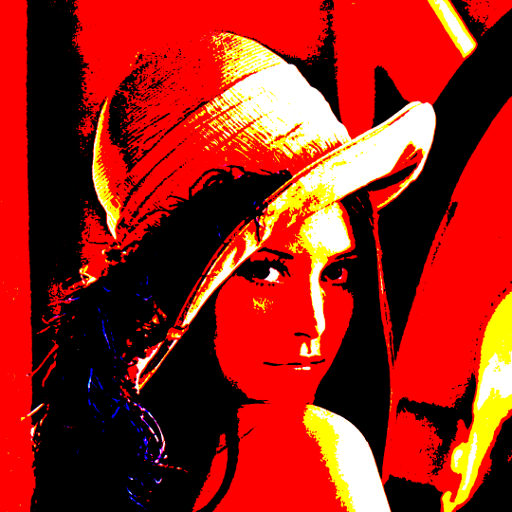
\includegraphics[width=\textwidth]{lena_filter_3}
        \caption{Tretji filter}
    \end{subfigure}
    \caption{Primerjava originalne slike z obdelano sliko}
    \label{fig:lena_filter_3}
\end{figure}


\subsubsection*{Filter 4}
Četrti filter je sestavljen iz dveh osnovnih filtrov. Najprej sliko obdelamo s
filtrom ``uravnovešanje barv'' in sicer s parametri $R = 100$, $G = -100$ in
$B = -100$. Rezultat obdelamo še s filtrom ``posteriziranje'' s parametrom
$ST = 3$. Rezultat testne slike lahko vidimo na sliki~\ref{fig:lena_filter_4}.

\begin{figure}[!ht]
    \centering
    \begin{subfigure}[b]{0.4\textwidth}
        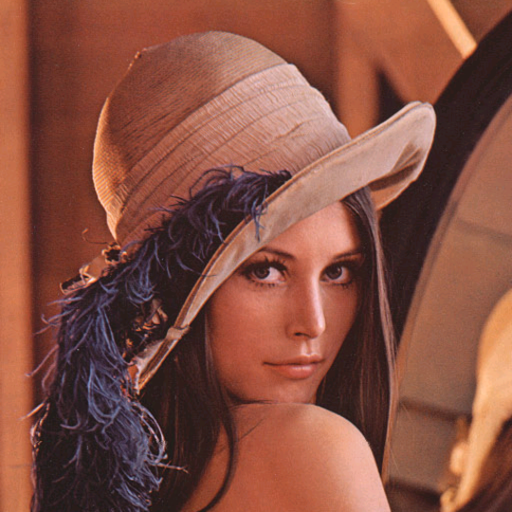
\includegraphics[width=\textwidth]{lena}
        \caption{Original}
    \end{subfigure}
    \begin{subfigure}[b]{0.4\textwidth}
        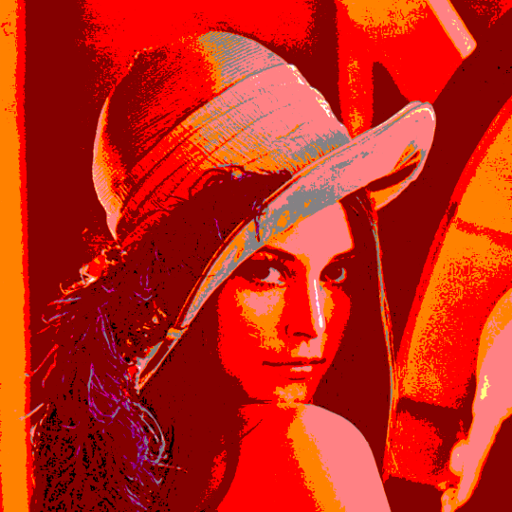
\includegraphics[width=\textwidth]{lena_filter_4}
        \caption{Četrti filter}
    \end{subfigure}
    \caption{Primerjava originalne slike z obdelano sliko}
    \label{fig:lena_filter_4}
\end{figure}


\subsubsection*{Filter 5}
Peti filter je sestavljen iz dveh osnovnih filtrov. Najprej sliko obdelamo s
filtrom ``uravnovešanje barv'' in sicer s parametri $R = -100$, $G = -100$ in
$B = 100$. Rezultat obdelamo še s filtrom ``posteriziranje'' s parametrom
$ST = 3$. Rezultat testne slike lahko vidimo na sliki~\ref{fig:lena_filter_5}.

\begin{figure}[!ht]
    \centering
    \begin{subfigure}[b]{0.4\textwidth}
        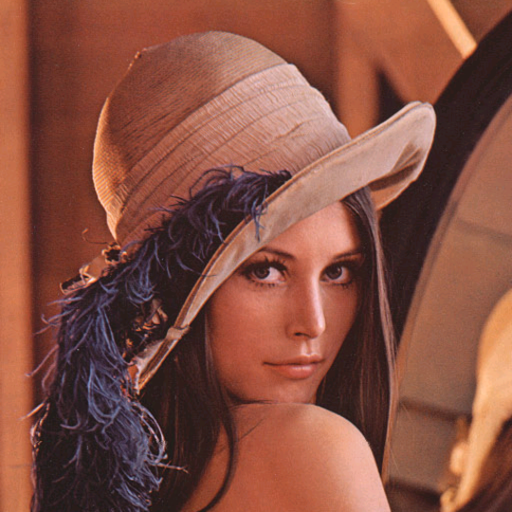
\includegraphics[width=\textwidth]{lena}
        \caption{Original}
    \end{subfigure}
    \begin{subfigure}[b]{0.4\textwidth}
        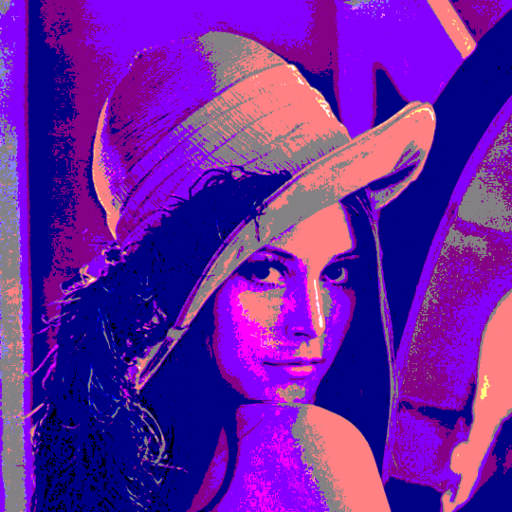
\includegraphics[width=\textwidth]{lena_filter_5}
        \caption{Peti filter}
    \end{subfigure}
    \caption{Primerjava originalne slike z obdelano sliko}
    \label{fig:lena_filter_5}
\end{figure}


\subsubsection*{Filter 6}
Šesti filter je sestavljen iz dveh osnovnih filtrov. Najprej sliko obdelamo s
filtrom ``uravnovešanje barv'' in sicer s parametri $R = -100$, $G = 100$ in
$B = -100$. Rezultat obdelamo še s filtrom ``posteriziranje'' s parametrom
$ST = 3$. Rezultat testne slike lahko vidimo na sliki~\ref{fig:lena_filter_6}.

\begin{figure}[!ht]
    \centering
    \begin{subfigure}[b]{0.4\textwidth}
        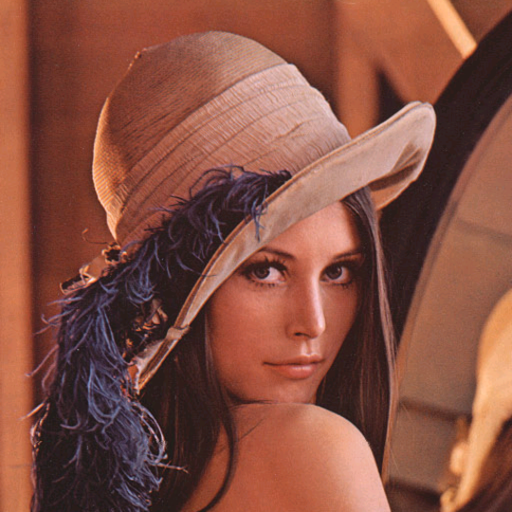
\includegraphics[width=\textwidth]{lena}
        \caption{Original}
    \end{subfigure}
    \begin{subfigure}[b]{0.4\textwidth}
        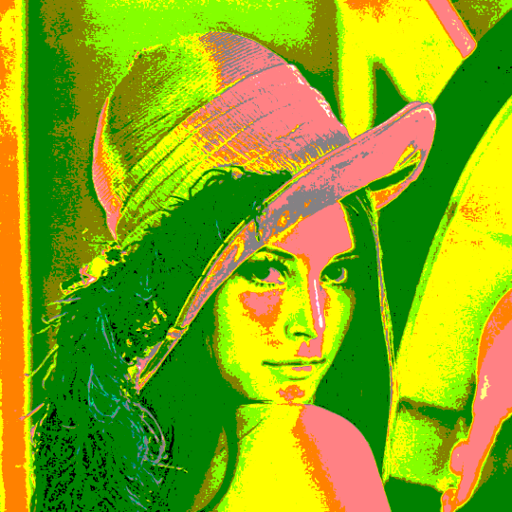
\includegraphics[width=\textwidth]{lena_filter_6}
        \caption{Šesti filter}
    \end{subfigure}
    \caption{Primerjava originalne slike z obdelano sliko}
    \label{fig:lena_filter_6}
\end{figure}


\subsubsection*{Filter 7}
Sedmi filter je sestavljen iz dveh osnovnih filtrov. Najprej sliko obdelamo s
filtrom ``posteriziranje'' in sicer s parametrom $ST = 5$. Rezultat obdelamo
še s filtrom ``uravnovešanje barv v HSL prostoru'' s parametri $H = -41$,
$L = -15$ in $S = 6$. Rezultat testne slike lahko vidimo na
sliki~\ref{fig:lena_filter_7}.

\begin{figure}[!ht]
    \centering
    \begin{subfigure}[b]{0.4\textwidth}
        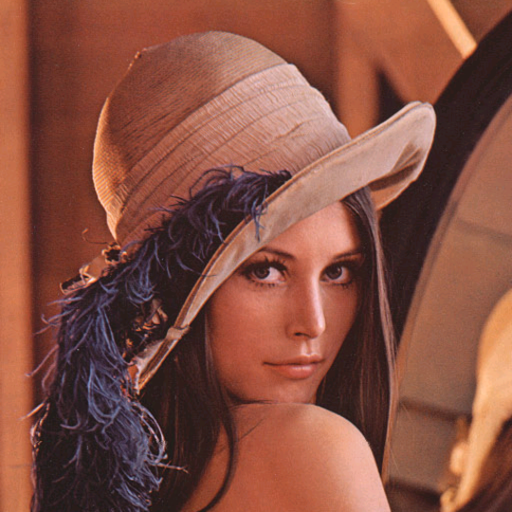
\includegraphics[width=\textwidth]{lena}
        \caption{Original}
    \end{subfigure}
    \begin{subfigure}[b]{0.4\textwidth}
        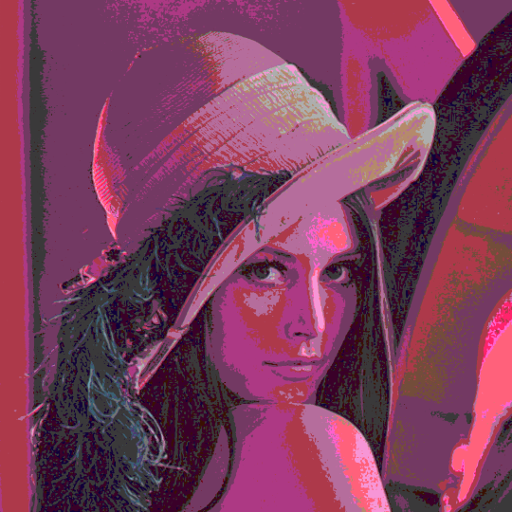
\includegraphics[width=\textwidth]{lena_filter_7}
        \caption{Sedmi filter}
    \end{subfigure}
    \caption{Primerjava originalne slike z obdelano sliko}
    \label{fig:lena_filter_7}
\end{figure}


\subsubsection*{Filter 8}
Osmi filter je sestavljen iz dveh osnovnih filtrov. Najprej sliko obdelamo s
filtrom ``posteriziranje'' in sicer s parametrom $ST = 6$. Rezultat obdelamo
še s filtrom ``uravnovešanje barv'' s parametri $R = -29$, $G = 40$ in $B = 100$.
Rezultat testne slike lahko vidimo na sliki~\ref{fig:lena_filter_8}.

\begin{figure}[!ht]
    \centering
    \begin{subfigure}[b]{0.4\textwidth}
        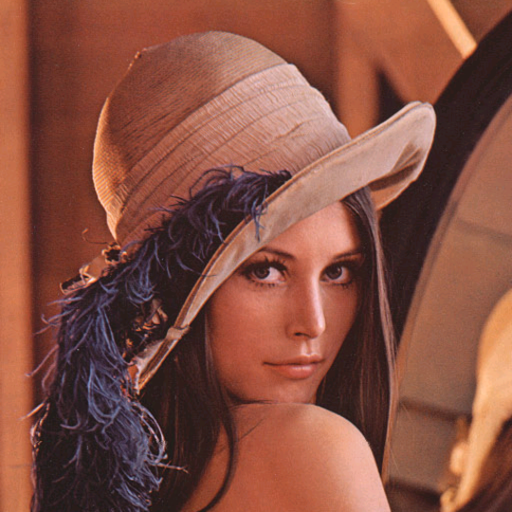
\includegraphics[width=\textwidth]{lena}
        \caption{Original}
    \end{subfigure}
    \begin{subfigure}[b]{0.4\textwidth}
        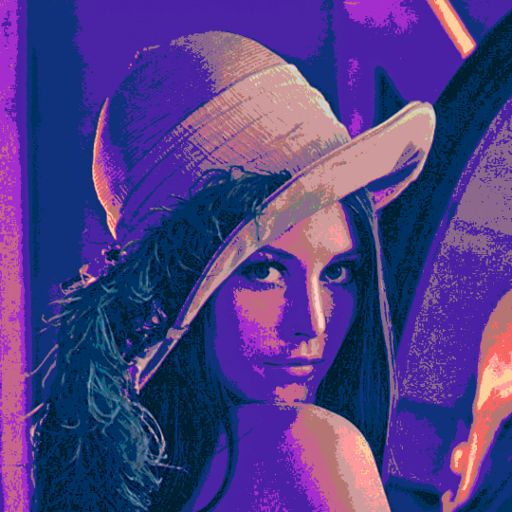
\includegraphics[width=\textwidth]{lena_filter_8}
        \caption{Osmi filter}
    \end{subfigure}
    \caption{Primerjava originalne slike z obdelano sliko}
    \label{fig:lena_filter_8}
\end{figure}


\subsubsection*{Filter 9}
Deveti filter je sestavljen iz dveh osnovnih filtrov. Najprej sliko obdelamo s
filtrom ``uravnovešanje barv v HSL prostoru'' in sicer s parametri $H = -41$,
$L = -20$ in $S = 25$. Rezultat obdelamo še s filtrom ``posteriziranje'' s
parametrom $ST = 4$. Rezultat testne slike lahko vidimo na
sliki~\ref{fig:lena_filter_9}.

\begin{figure}[!ht]
    \centering
    \begin{subfigure}[b]{0.4\textwidth}
        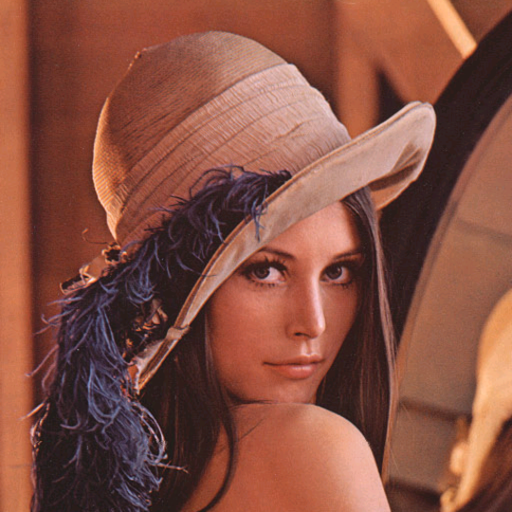
\includegraphics[width=\textwidth]{lena}
        \caption{Original}
    \end{subfigure}
    \begin{subfigure}[b]{0.4\textwidth}
        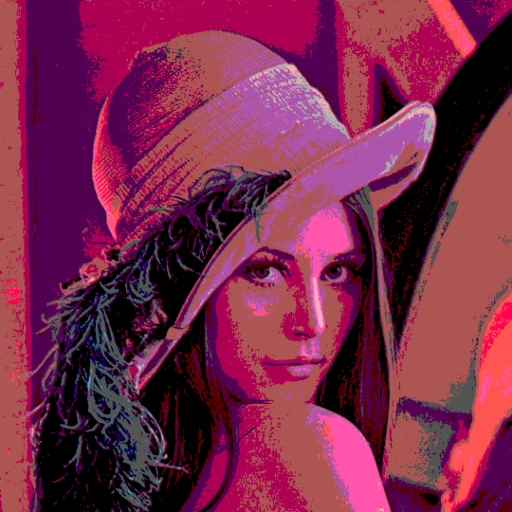
\includegraphics[width=\textwidth]{lena_filter_9}
        \caption{Deveti filter}
    \end{subfigure}
    \caption{Primerjava originalne slike z obdelano sliko}
    \label{fig:lena_filter_9}
\end{figure}


\subsubsection*{Filter 10}
Deseti filter je sestavljen iz treh osnovnih filtrov. Najprej sliko obdelamo s
filtrom ``uravnovešanje barv'' in sicer s parametri $R = 100$, $G = -100$ in
$B = -100$. Rezultat obdelamo še s filtrom ``posteriziranje'' s parametrom
$ST= 3$ in nazadnje še s filtrom ``uravnovešanje barv v HSL prostoru'' s
parametri $H = -41$, $L = -10$ in $S = 20$. Rezultat testne slike lahko
vidimo na sliki~\ref{fig:lena_filter_10}.

\begin{figure}[!ht]
    \centering
    \begin{subfigure}[b]{0.4\textwidth}
        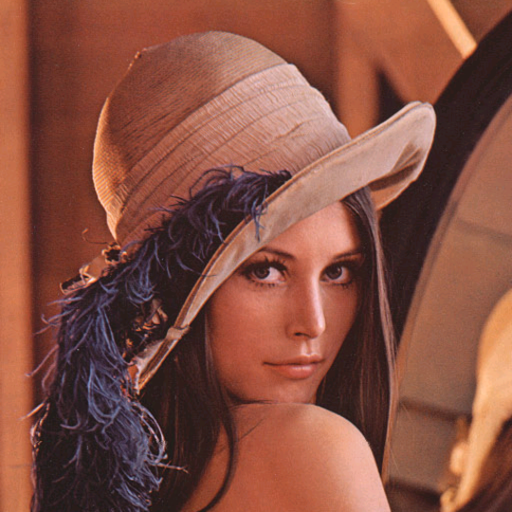
\includegraphics[width=\textwidth]{lena}
        \caption{Original}
    \end{subfigure}
    \begin{subfigure}[b]{0.4\textwidth}
        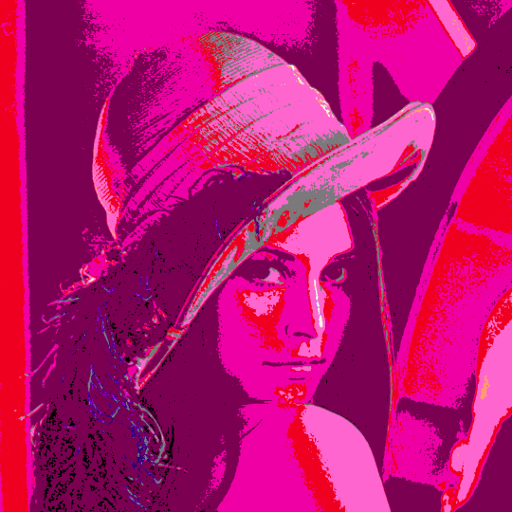
\includegraphics[width=\textwidth]{lena_filter_10}
        \caption{Deseti filter}
    \end{subfigure}
    \caption{Primerjava originalne slike z obdelano sliko}
    \label{fig:lena_filter_10}
\end{figure}


\subsubsection*{Filter 11}
Enajsti filter je sestavljen iz treh osnovnih filtrov. Najprej sliko obdelamo s
filtrom ``uravnovešanje barv'' in sicer s parametri $R = 34$, $G = -38$ in
$B = 24$. Rezultat obdelamo še s filtrom ``posteriziranje'' s parametrom
$ST= 4$ in nazadnje še s filtrom ``uravnovešanje barv v HSL prostoru'' s
parametri $H = -65$, $L = 0$ in $S = 0$. Rezultat testne slike lahko
vidimo na sliki~\ref{fig:lena_filter_11}.

\begin{figure}[!ht]
    \centering
    \begin{subfigure}[b]{0.4\textwidth}
        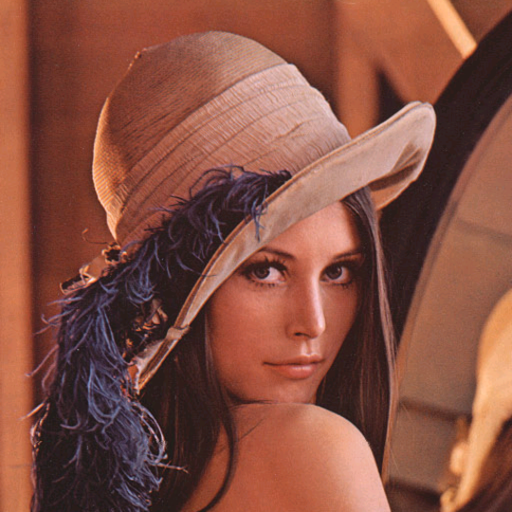
\includegraphics[width=\textwidth]{lena}
        \caption{Original}
    \end{subfigure}
    \begin{subfigure}[b]{0.4\textwidth}
        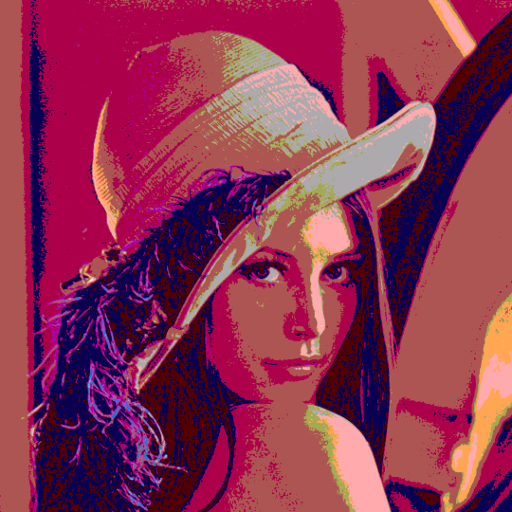
\includegraphics[width=\textwidth]{lena_filter_11}
        \caption{Enajsti filter}
    \end{subfigure}
    \caption{Primerjava originalne slike z obdelano sliko}
    \label{fig:lena_filter_11}
\end{figure}


\subsubsection*{Filter 12}
Dvanajsti filter je sestavljen iz dveh osnovnih filtrov. Najprej sliko obdelamo s
filtrom ``uravnovešanje barv'' in sicer s parametri $R = 40$, $G = -40$ in
$B = 28$. Rezultat obdelamo še s filtrom ``posteriziranje'' s parametrom
$ST= 4$ in nazadnje še enkrat s filtrom ``uravnovešanje barv'' vendar s
parametri $R = -100$, $G = -42$ in $B = 100$. Rezultat testne slike lahko
vidimo na sliki~\ref{fig:lena_filter_12}.

\begin{figure}[!ht]
    \centering
    \begin{subfigure}[b]{0.4\textwidth}
        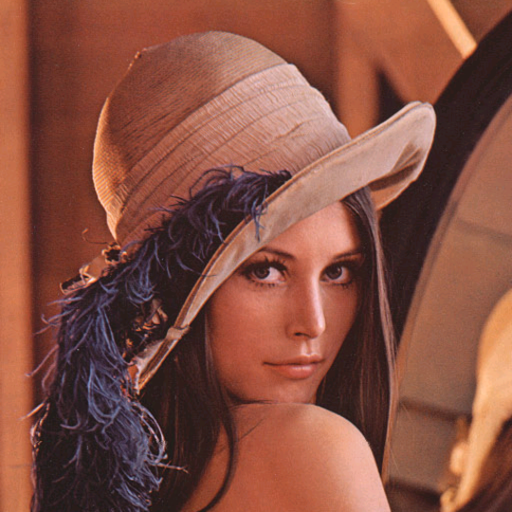
\includegraphics[width=\textwidth]{lena}
        \caption{Original}
    \end{subfigure}
    \begin{subfigure}[b]{0.4\textwidth}
        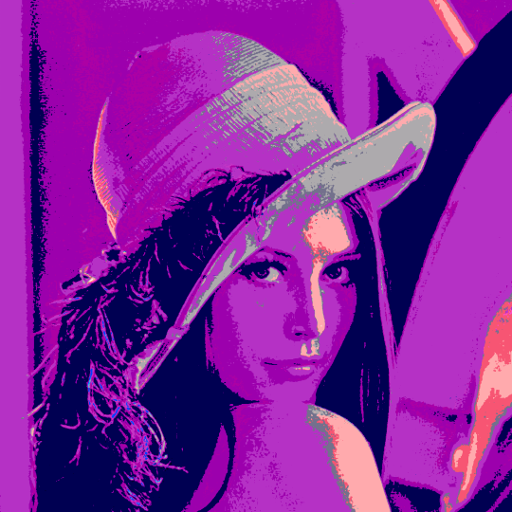
\includegraphics[width=\textwidth]{lena_filter_12}
        \caption{Dvanajsti filter}
    \end{subfigure}
    \caption{Primerjava originalne slike z obdelano sliko}
    \label{fig:lena_filter_12}
\end{figure}


\subsubsection*{Filter 13}
Trinajsti filter je sestavljen iz dveh osnovnih filtrov. Najprej sliko obdelamo s
filtrom ``uravnovešanje barv'' in sicer s parametri $R = 45$, $G = -45$ in
$B = 35$. Rezultat obdelamo še s filtrom ``posteriziranje'' s parametrom
$ST =4$. Rezultat testne slike lahko vidimo na sliki~\ref{fig:lena_filter_13}.

\begin{figure}[!ht]
    \centering
    \begin{subfigure}[b]{0.4\textwidth}
        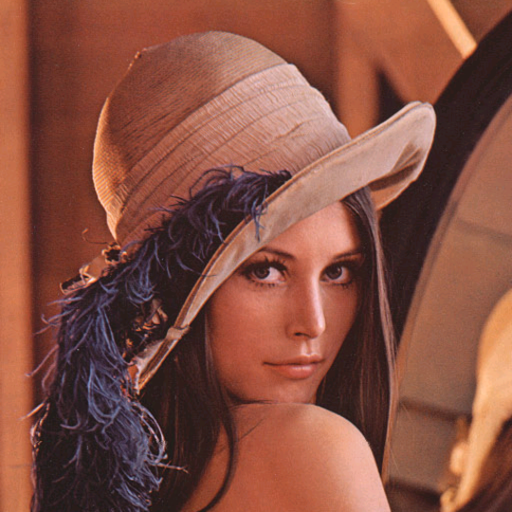
\includegraphics[width=\textwidth]{lena}
        \caption{Original}
    \end{subfigure}
    \begin{subfigure}[b]{0.4\textwidth}
        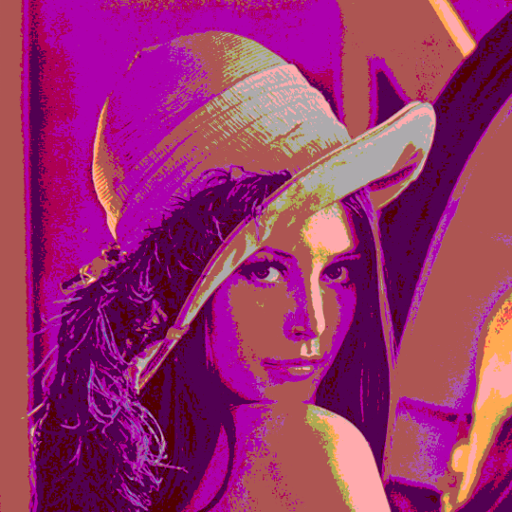
\includegraphics[width=\textwidth]{lena_filter_13}
        \caption{Trinajsti filter}
    \end{subfigure}
    \caption{Primerjava originalne slike z obdelano sliko}
    \label{fig:lena_filter_13}
\end{figure}


\subsubsection*{Filter 14}
Štirinajsti filter je sestavljen iz dveh osnovnih filtrov. Najprej sliko obdelamo s
filtrom ``uravnovešanje barv'' in sicer s parametri $R = -45$, $G = -55$ in
$B = 30$. Rezultat obdelamo še s filtrom ``posteriziranje'' s parametrom
$ST =4$. Rezultat testne slike lahko vidimo na sliki~\ref{fig:lena_filter_14}.

\begin{figure}[!ht]
    \centering
    \begin{subfigure}[b]{0.4\textwidth}
        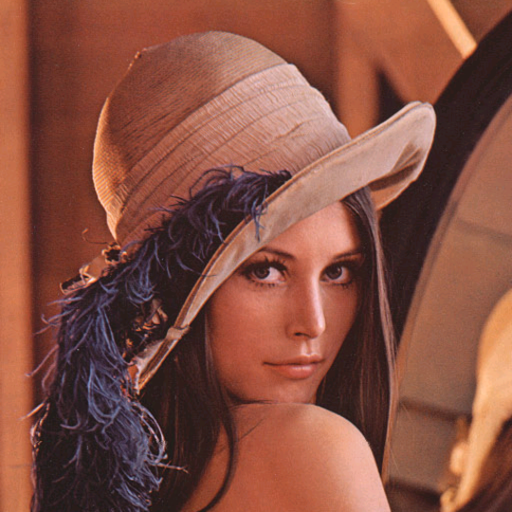
\includegraphics[width=\textwidth]{lena}
        \caption{Original}
    \end{subfigure}
    \begin{subfigure}[b]{0.4\textwidth}
        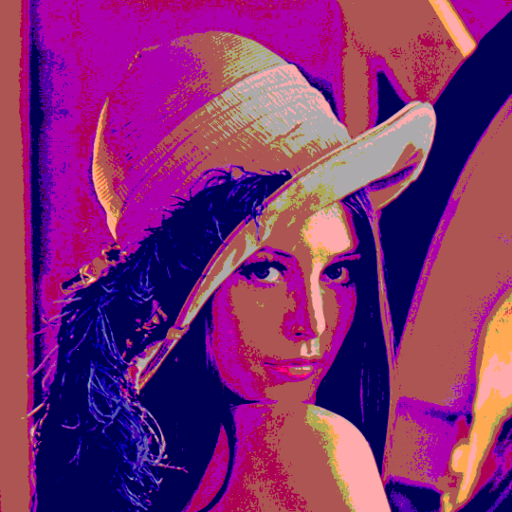
\includegraphics[width=\textwidth]{lena_filter_14}
        \caption{Štirinajsti filter}
    \end{subfigure}
    \caption{Primerjava originalne slike z obdelano sliko}
    \label{fig:lena_filter_14}
\end{figure}


\subsubsection*{Filter 15}
Petnajsti filter vsebuje le osnovni filter ``posteriziranje'' in sicer s parametrom
$ST = 3$. Rezultat testne slike lahko vidimo na sliki~\ref{fig:lena_filter_15}.

\begin{figure}[!ht]
    \centering
    \begin{subfigure}[b]{0.4\textwidth}
        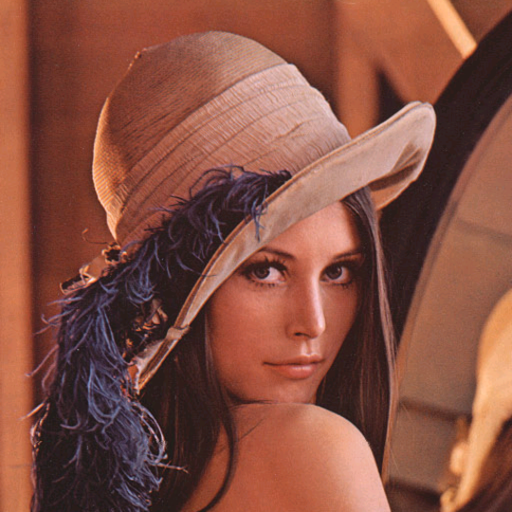
\includegraphics[width=\textwidth]{lena}
        \caption{Original}
    \end{subfigure}
    \begin{subfigure}[b]{0.4\textwidth}
        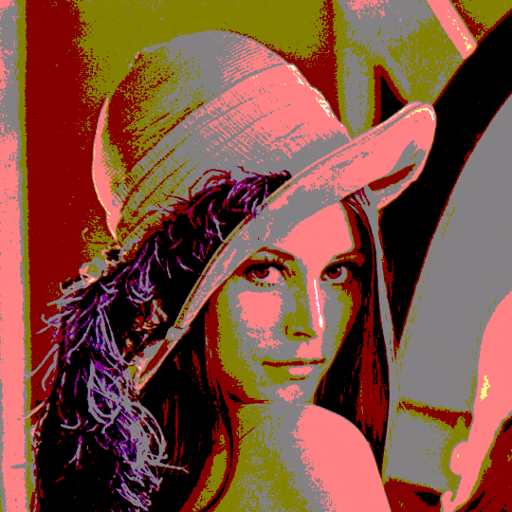
\includegraphics[width=\textwidth]{lena_filter_15}
        \caption{Petnajsti filter}
    \end{subfigure}
    \caption{Primerjava originalne slike z obdelano sliko}
    \label{fig:lena_filter_15}
\end{figure}


\subsubsection*{Filter 16}
Šestnajsti filter je sestavljen iz dveh osnovnih filtrov. Najprej sliko obdelamo s
filtrom ``uravnovešanje barv'' in sicer s parametri $R = 30$, $G = -40$ in
$B = 16$. Rezultat obdelamo še s filtrom ``posteriziranje'' s parametrom
$ST =3$. Rezultat testne slike lahko vidimo na sliki~\ref{fig:lena_filter_16}.

\begin{figure}[!ht]
    \centering
    \begin{subfigure}[b]{0.4\textwidth}
        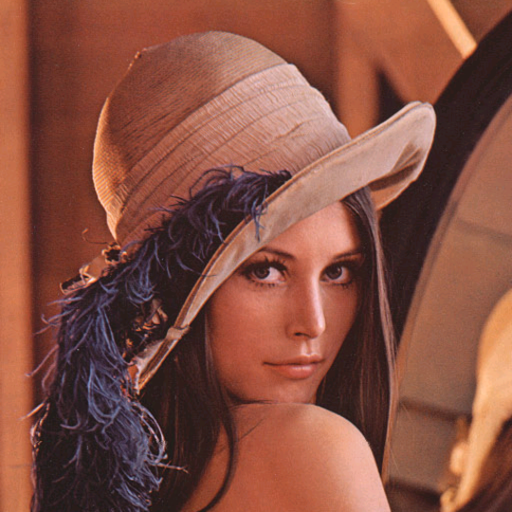
\includegraphics[width=\textwidth]{lena}
        \caption{Original}
    \end{subfigure}
    \begin{subfigure}[b]{0.4\textwidth}
        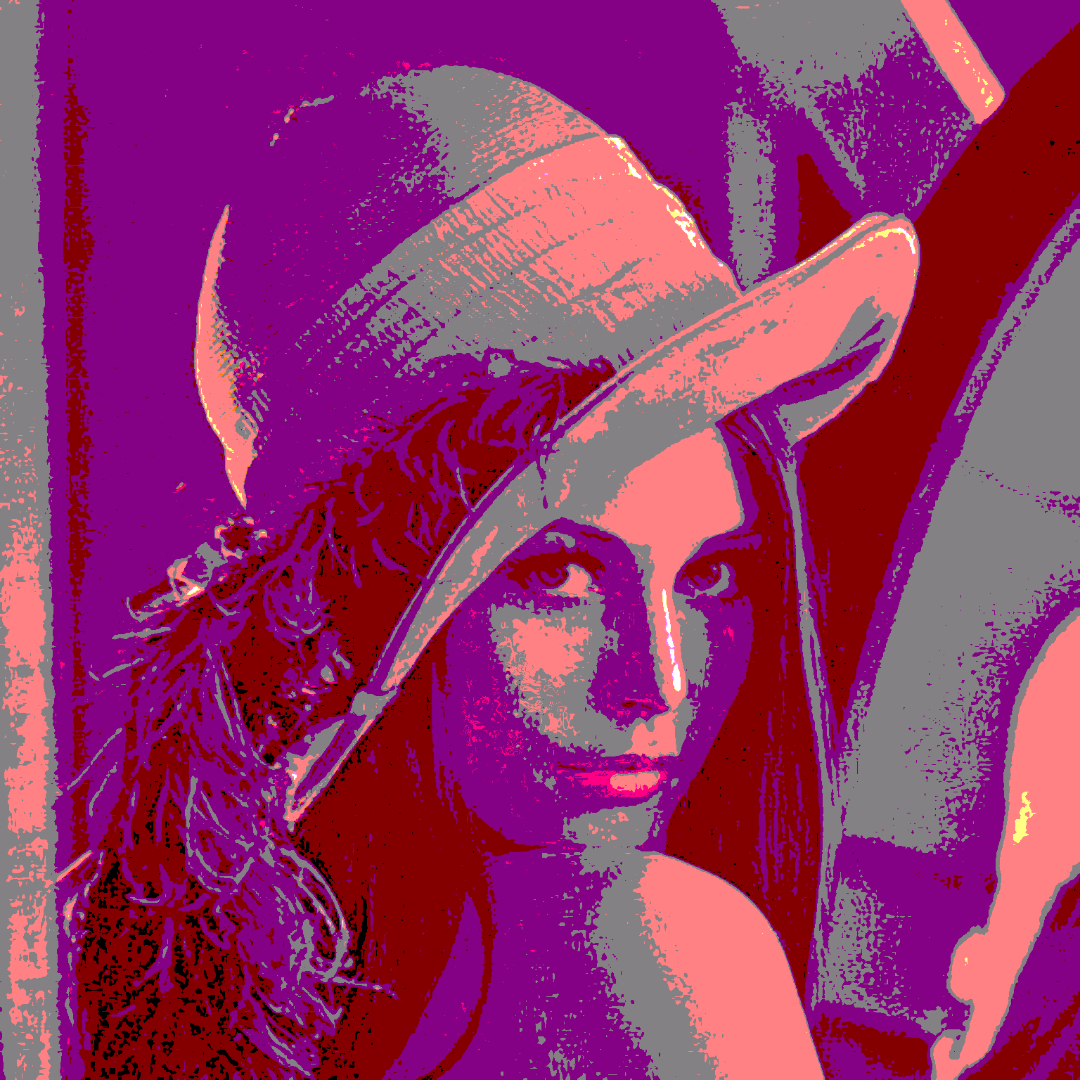
\includegraphics[width=\textwidth]{lena_filter_16}
        \caption{Šestnajsti filter}
    \end{subfigure}
    \caption{Primerjava originalne slike z obdelano sliko}
    \label{fig:lena_filter_16}
\end{figure}


\subsubsection*{Filter 17}
Sedemnajsti filter je sestavljen iz treh osnovnih filtrov. Najprej sliko obdelamo s
filtrom ``uravnovešanje barv'' in sicer s parametri $R = 20$, $G = -30$ in
$B = 20$. Rezultat obdelamo še s filtrom ``posteriziranje'' s parametrom
$ST= 4$ in nazadnje še s filtrom ``uravnovešanje barv v HSL prostoru'' s
parametri $H = -30$, $L = -10$ in $S = 12$. Rezultat testne slike lahko
vidimo na sliki~\ref{fig:lena_filter_17}.

\begin{figure}[!ht]
    \centering
    \begin{subfigure}[b]{0.4\textwidth}
        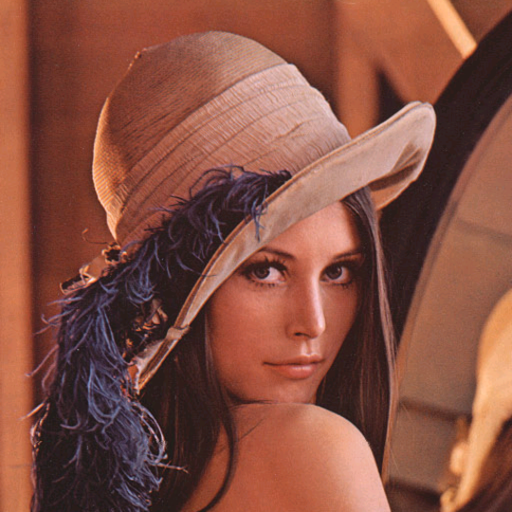
\includegraphics[width=\textwidth]{lena}
        \caption{Original}
    \end{subfigure}
    \begin{subfigure}[b]{0.4\textwidth}
        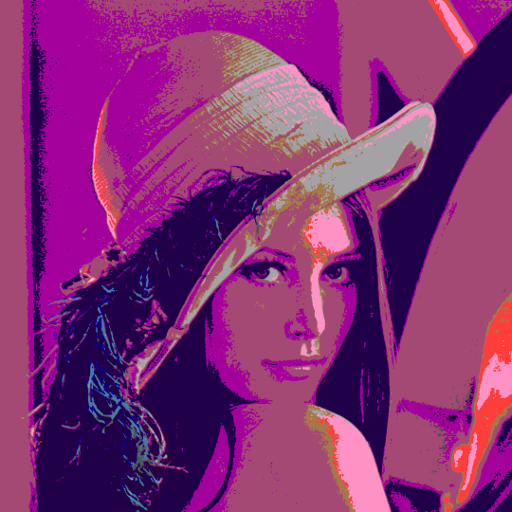
\includegraphics[width=\textwidth]{lena_filter_17}
        \caption{Sedemnajsti filter}
    \end{subfigure}
    \caption{Primerjava originalne slike z obdelano sliko}
    \label{fig:lena_filter_17}
\end{figure}


\chapter{Nove funkcionalne možnosti}


\chapter{Povezovanje s socialnimi omrežji}
Ena izmed pomembnejših posodobitev je povezava s socialnimi omrežji, ki so
vsak dan bolj popularni. Vsak dan se na različnih socialnih omrežjih doda na
tisoče žargonsko imenovanih ``selfijev''\footnote{Slika, ko oseba fotografira
samega sebe pri različnih dejavnostih.}. Da pa ta ``selfi'' še bolj pade v
oči, se jim lahko doda kakšen že vnaprej določen filter. Ti so pri pametnih
telefonih, ki je danes eden izmed najpogostejših naprav za fotografiranje
``selfijev'', na voljo samo en dotik stran. Obstajajo pa tudi že socialna
omrežja, ki ponujajo osnovne filtre že pri nalaganju slike.

Naša instalacija se lahko interpretira kot generator ``selfijev''. Oseba, ki stoji pred
instalacijo, ve, da bo kmalu njenih petnajst sekund. Pred njo se bo pokazala
pop-art slika, ki je njen umetniški ``selfi'', in če želi, je ta pop-art slika
lahko kmalu javna na enem izmed socialnih omrežij.


\section{Možnosti}
\section{Omejitve}
TODO: PREVERI KAJ JE RES IN KAJ NE
Ena izmed največjih omejitev je nenadzorovano pošiljanje slik na socialno
omrežje. Na slikah so lahko osebe, ki si ne želijo biti objavljeni na
socialnem omrežju, saj je javno. Še več, na slikah so lahko otroci, katerih
objavljanje slik na socialnem omrežju je prepovedano brez dovoljenja staršev.
Res je, da smo želeli slike izbrisati petnajst sekund po pojavi, vendar pa
večina socialnih omrežjih te slike še vedno hrani, čeprav jih ne vidimo več.
In če se podamo v najhujšo skrajnost, napisati program, ki vse slike shranjuje
na nek strežnik.


% \chapter{TODO}
% Datoteka {\tt magistrska\_naloga.tex} na kratko opisuje, kako se pisanja
% magistrskega dela lotimo z uporabo programskega pateka \LaTeX. V tem dokumentu
% bomo predstavili nekaj njegovih prednosti in hib. Kar se slednjih tiče, mi
% pride na misel ena sama. Ko se srečamo z njim, nam izgleda kot kislo jabolko,
% nismo prepričani, da bi želeli vanj ugrizniti. Lahko pa z njim pripravimo
% odličen zavitek ali pa pridemo na okus.

% Česa od tega dokumenta ne pričakujte? Izkušeni uporabniki \LaTeX{}a bi vse
% skupaj zastavili drugače. Morda bi napisali posebno razredno datoteko
% (\emph{class file}) --- v resnici priredili katero od obstoječih ---, v
% datoteki {\tt magistrska\_naloga.tex} ohranili samo najbolj grobo strukturo in
% vanjo vključevali  posamezna po\-glav\-ja. Hkrati s pisanjem teksta bi
% poskrbeli tudi za stvarno kazalo ({\tt makeindex}), literaturo pa bi citirali
% z uporabo {\BibTeX}{a}. Tega, skratka, v tem dokumentu ne boste našli.

% Kaj vseeno najdemo. V Poglavju~\ref{ch1} bomo na hitro spoznali besedilne
% konstrukte kot so izreki, enačbe in dokazi. Naučili se bomo, kako se na njih
% sklicujemo. Poglavje~\ref{ch2} bo predstavilo vključevanje plovk: slik in
% tabel. V Poglavju~\ref{ch3} se bomo srečali s sklicevanjem na literaturo.
% Sledil bo samo še zaključek.

% \chapter{Sklicevanje na besedilne konstrukte}
% \label{ch1}
% Matematična ali popolna indukcija je eno prvih orodij, ki jih spoznamo za dokazovanje trditev pri matematičnih predmetih.
% \begin{izrek}
% \label{iz:1}
% Za vsako naravno število $n$ velja
% \begin{equation}
% n < 2^n.
% \label{eq:1}
% \end{equation}
% \end{izrek}
% \begin{dokaz}
% Dokazovanje z indukcijo zahteva, da neenakost~\eqref{eq:1} najprej preverimo za najmanjše naravno število --- $0$. Res, ker je $0 < 1 = 2^0$, je neenačba~\eqref{eq:1} za $n=0$ izpolnjena.

% Sledi indukcijski korak. S predpostavko, da je neenakost~\eqref{eq:1} veljavna pri nekem naravnem številu $n$, je potrebno pokazati, da je ista neenakost v veljavi tudi pri njegovem nasledniku --- naravnem številu $n+1$. Računajmo.
% \begin{align}
% n+1 &< 2^n + 1  \label{eq:2}\\
%     &\le 2^n + 2^n \label{eq:3}\\
%     &= 2^{n+1} \nonumber
% \end{align}
% Neenakost~\eqref{eq:2} je posledica indukcijske predpostavke, neenakost~\eqref{eq:3} pa enostavno dejstvo, da je za vsako naravno število $n$ izraz $2^n$ vsaj tako velik kot 1. S tem je dokaz Izreka~\ref{iz:1} zaključen.
% \end{dokaz}

% Opazimo, da je \LaTeX\ številko izreka podredil številki poglavja.


% \chapter{Plovke: slike in tabele}
% \label{ch2}
% Slike in daljše tabele praviloma vključujemo v dokument kot plovke. Pozicija plovke v končnem izdelku ni pogojena s tekom besedila, temveč z izgledom strani. \LaTeX\ bo skušal plovko postaviti samostojno, praviloma na vrh strani, na kateri se na takšno plovko prvič sklicujemo. Pri tem pa bo na vsako stran končnega izdelka želel postaviti tudi sorazmerno velik del besedila. V skrajnem primeru, če imamo res preveč plovk, se bo odločil za stran popolnoma zapolnjeno s plovkami.

% \section{Formati slik}
% Bitne slike, vektorske slike, kakršnekoli slike, z \LaTeX{}om lahko vključimo vse.
% Slika~\ref{pic1} je v {\tt .pdf} formatu.
% \begin{figure}
%     \begin{center}
%         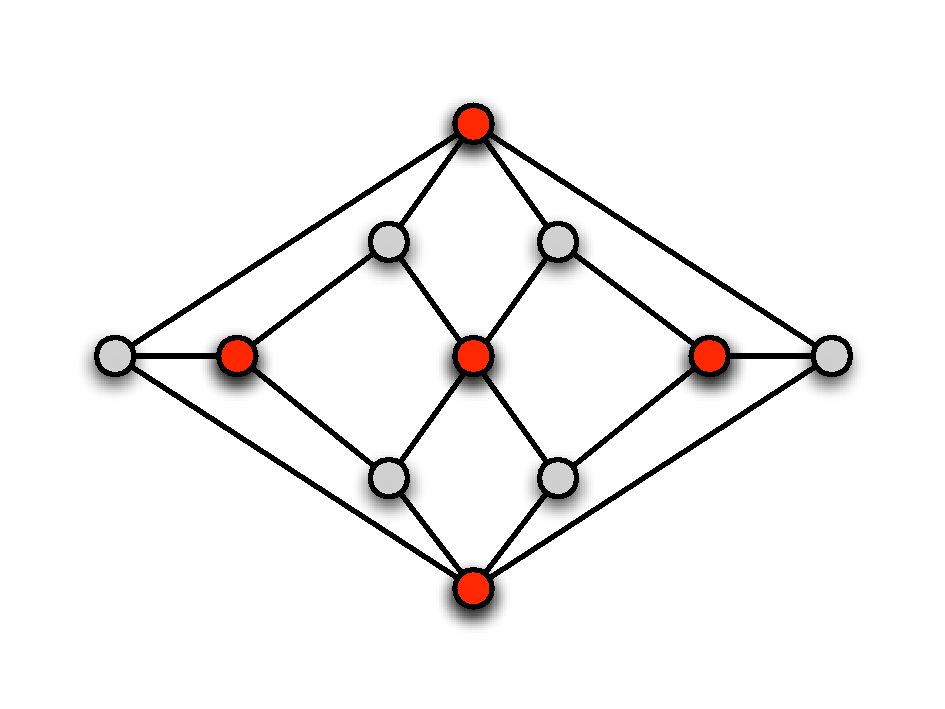
\includegraphics[width=10cm]{pic1.pdf}
%     \end{center}
% \caption{Herschelov graf, vektorska grafika.}
% \label{pic1}
% \end{figure}
% Pa res lahko vključimo slike katerihkoli formatov? Žal ne. Programski paket \LaTeX\ lahko uporabljamo v več dialektih. Ukaz {\tt latex} ne mara vključenih slik v formatu Portable Document Format {\tt .pdf}, ukaz {\tt pdflatex} pa ne prebavi slik v Encapsulated Postscript Formatu {\tt .eps}.
% Strnjeno v Tabeli~\ref{tbl:1}.

% \begin{table}
%     \begin{center}
%         \begin{tabular}{l|ccc}
%             ukaz/format & {\tt .pdf} & {\tt .eps} & ostali formati \\ \hline
%                         {\tt pdflatex} & da & ne & da \\
%                         {\tt latex}   & ne & da  & da
%         \end{tabular}
%     \end{center}
% \caption{}
% \label{tbl:1}
% \end{table}

% Nasvet? Odločite se za uporabo ukaza {\tt pdflatex}. Vaš izdelek bo brez vmesnih stopenj na voljo v {.pdf} formatu in ga lahko odnesete v vsako tiskarno. Če morate na vsak način vključiti sliko, ki jo imate v {\tt .eps} formatu, jo vnaprej pretvorite v alternativni format, denimo {\tt .pdf}.

% Včasih se da v okolju za uporabo programskega paketa \LaTeX\ nastaviti na kakšen način bomo prebavljali vhodne dokumente. Spustni meni na Sliki~\ref{pic2} odkriva uporabo \LaTeX{}a v njegovi pdf inkarnaciji --- {\tt pdflatex}.
% \begin{figure}
% \begin{center}
% 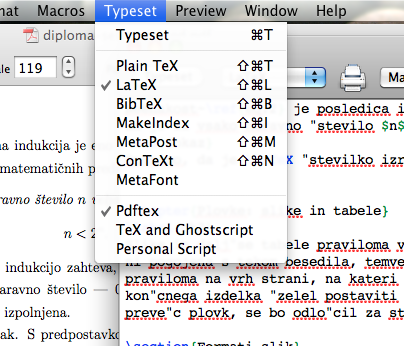
\includegraphics[width=10cm]{pic2.png}
% \end{center}
% \caption{Kateri dialekt uporabljati?}
% \label{pic2}
% \end{figure}

% Vključena Slika~\ref{pic2} je seveda bitna.

% Kaj pa stran iz študentskega referata?\label{pp}
% Tudi njo lahko vključimo v dokument. Toda ne kot plovko.


% \chapter{Kaj pa literatura?}
% \label{ch3}
% Kot smo omenili že v uvodu, je pravi način za citiranje literature uporaba \BibTeX{}a~\cite{bib}.
% Programski paket \LaTeX je prvotno predstavljen v priročniku~\cite{lat} in je v resnici nadgradnja sistema \TeX\ avtorja Donalda Knutha, znanega po denimo, če izpustim njegovo umetnost programiranja, Knuth-Bendixovem algoritmu~\cite{dk1}.

% Vsem raziskovalcem s področja računalništva pa svetujem v branje mnenje L.\ Fortnowa~\cite{lf}~\cite{trifonova}.

\chapter{Sklepne ugotovitve}
Izbira \LaTeX\ ali ne \LaTeX\ je seveda prepuščena vam samim. Res je, da so prvi koraki v \LaTeX{}u težavni. Ta dokument naj vam služi kot začetna opora pri hoji.
